
\chapter{Introducción} \label{intro}
	
	\section{Contexto} \label{context}
	
	%	TESIS EUGENIO:
	%	Desarrollar aqui el comportamiento humano -> pedir / hacer opiniones
	%	Evolución histórica de la opinión -> Hasta web 2.0
	
	La principal característica del ser humano y la que le diferencia del resto de seres vivos es la racionalidad. El ser humano utiliza la razón para la toma de decisiones, contemplando los diferentes escenarios y evaluando la mejor manera de alcanzar sus objetivos. Sin embargo, el ser humano consta de una racionalidad limitada, por lo que el abanico de posibilidades que baraja en cada momento está limitado por su visión de la realidad. 
	
	Es por esto que el proceso de toma de decisiones constituye un gran reto. Para facilitar el proceso de toma de decisiones y con el fin de ampliar el abanico de consecuencias contempladas, es muy común la acción de ``pedir opinión'' a terceros.
	
	 La ayuda en la toma de decisiones no es la única función de las opiniones. Las personas también utilizamos las opiniones para expresar nuestro juicio acerca de variados temas. Cuando se produce un intercambio de opiniones ambos participantes se enriquecen con el punto de vista del contrario. 
	 
	El uso de las opiniones ha evolucionado con el ser humano a lo largo de la historia. Comenzando en los inicios del lenguaje, pasando a estar por escrito con la llegada de la escritura y disparándose con el auge de la difusión de opinión en la prensa con la invención del a imprenta.
	
	Uno de los acontecimientos más influyentes en la sociedad fue la invención de Internet en la segunda mitad del s. XX. Trajo consigo una gran fuente de información de fácil acceso. A principios del s.XXI enfatizó el cambio social que ya estaba ocurriendo un nuevo concepto de Web, la Web 2.0. Este innovador concepto ofrecía a todo usuario de ella la posibilidad de compartir todo tipo de información en Internet. Así fue como se preparó el camino para la llegada de las redes sociales, los blogs, o los foros. Plataformas donde los usuarios podían compartir todo tipo de pensamientos u opiniones sin ningún flitro. También se sumaron al carro de la Web 2.0 las empresas. Muchas de ellas incorporaron la opción de compra \textit{online} suponiendo una nueva fuente de ingresos e incluso surgieron muchas nuevas empresas que llevan a cabo toda su funcionalidad a través de Internet.
	
	%Poner aquí una frase final que no se quede como en el aire 

	
	\section{Motivación} \label{motivacion}
	%	TFG MIGUEL:
	%	Conectando con lo anterior -> hay muchísimas opiniones en internet
	%	Aparición de grandes empresas
	%	Las empresas quieren/necesitan conocer la opinión/éxito/fracaso de sus productos 
	%	para los procesos de marketing y para posibles mejoras

	En el contexto de la Sección \ref{context}, tanto el auge de las redes sociales como la incorporación de las empresas al negocio \textit{online} no trajeron consigo solo nuevas fuentes de beneficios. La Web 2.0 supuso una nueva (y enorme) fuente de información. Esta generación exponencial de datos de naturaleza desestructurada en Internet propició el nacimiento de lo que hoy conocemos como \textit{Big Data}.
	
	\begin{figure}[h!]
		\centering
		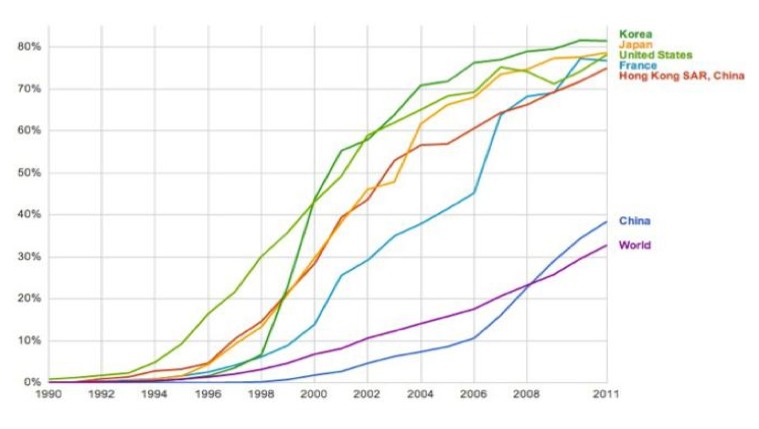
\includegraphics[width=0.7\linewidth]{imagenes/grafica-intro}
		\caption{Gráfica del crecimiento del \textit{Big Data} en algunos países y en el mundo.}
		\label{fig:grafica-intro}
	\end{figure}
	 
	 Para hacernos una idea del impacto del nacimiento de la Web 2.0, observamos la Figura \ref{fig:grafica-intro} en la que se representa el crecimiento de \textit{Big Data} en algunos países desarrollados y en el mundo en general. Notamos que en el año 1998 se produce un aumento en el ritmo de crecimiento, coincidiendo con el nacimiento de la Web 2.0. El siguiente cambio de crecimiento más brusco lo encontramos en el año 2006, año de mayor impacto de las redes sociales. 
	 
	 %Quizás nombrar en algún momento microblogging (Twitter) y esop
	 
	 Como ya veníamos advirtiendo, está en la naturaleza del ser humano dar su opinión sobre los temas que le rodean. Esta caracterización del ser humano junto con la cantidad de datos depositados por usuarios en los diferentes portales de Internet nos da una idea de la cantidad de opiniones disponibles. Esta información será de gran utilidad para las empresas que quieran conocer la opinión de los usuarios sobre un determinado producto o, simplemente, para conocer la opinión de la población sobre un determinado tema.  Sin embargo, la inmensurable cantidad de información disponible hace que contratar a personal especializado para que se dedique a estudiar las opiniones de un determinado producto o tema de actualidad sería inviable tanto desde el punto de vista económico como desde el temporal.  Debido a la necesidad de monitorizar este procedimiento surge el concepto de Análisis de Sentimientos o Minería de Opinión, del que hablaremos en los siguientes capítulos.
	 
	 Por su estructura de \textit{microblogging} (red social con un número de caracteres limitados para resaltar la opinión), Twitter es un perfecto generador de opiniones para analizar mediante Análisis de Sentimientos. Ya se han llevado a cabo estudios sobre esta plataforma obteniendo muy buenos resultados. Por ejemplo, en las últimas elecciones presidenciales de EEUU se realizó un estudio sobre la opinión de los usuarios de Twitter sobre ambos candidatos. Para este estudio se utilizaron los tweets publicados hasta 43 días antes de las elecciones comenzando el primer día de candidatura. Utilizando expertos para el etiquetado de los datos como positivos o negativos referentes a cada uno de los candidatos y entrenando con un algoritmo de Naïve Bayes consiguieron un 94\% de correlación.
	 
	 El término de Análisis de Sentimientos es un término relativamente reciente. Aunque ya haya tenido éxito en algunos ámbitos, es un campo aún sin explotar pues presenta dificultades que aún no han sido solventadas.  Entre estas dificultades se encuentran la subjetividad de las opiniones, las particularidades del lenguaje, los contextos, los sarcasmos ... entre una interminable lista.
	 
	 
	 \begin{figure}[h!]
	 	\centering
	 	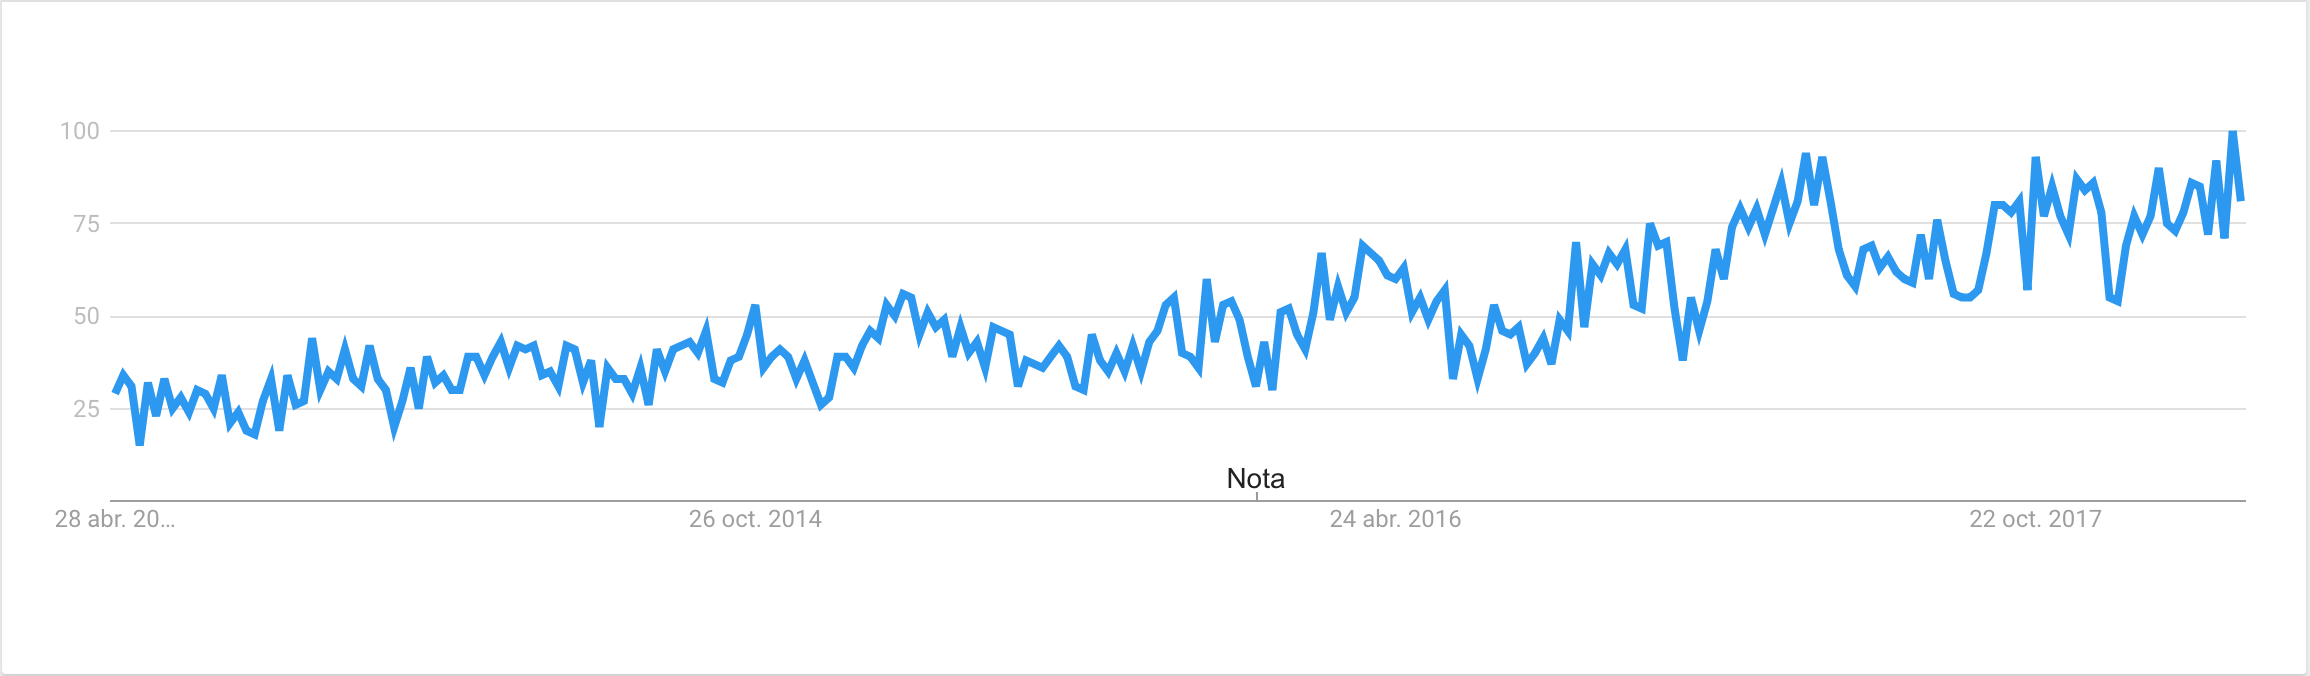
\includegraphics[width=1\linewidth]{imagenes/interes}
	 	\caption{Gráfica que representa el interés del análisis de sentimientos en todo el mundo según Google Trends.}
	 	\label{fig:interes}
	 \end{figure}
	 
	 Esto hace que se presente como una campo de estudio muy llamativo, con muchas mejoras por hacer y con un futuro muy prometedor. Cada día más gente centra su interés en esta materia (Figura \ref{fig:interes}). De ahí que a lo largo de esta memoria nos dediquemos al estudio de una parte de este amplio campo.
	 

	Como ya podemos imaginar, el término Análisis de Sentimientos abarca un gran conjunto de tareas. El trabajo se va a centrar en una de esas tareas en concreto: la extracción de características. 

	Para explicar en qué consiste y su importancia, trabajaremos sobre un ejemplo concreto. Imaginemos que queremos analizar la siguiente opinión:
	
	\begin{center}
		\begin{minipage}{0.9\linewidth}
			\vspace{5pt}%margen superior de minipage
			{\small
				[1] \textit{El ordenador tiene muy buen procesador, sin embargo la pantalla tiene poca resolución y el precio es muy elevado.}
			}
			\vspace{5pt}%margen inferior de la minipage
		\end{minipage}
	\end{center}

	Si tuviéramos que establecer una polaridad a dichar frase, sería una tarea complicada incluso para una persona. En la frase se nombran tres componentes de un mismo ordenador y se da un opinión sobre cada una de ellas. Así, \textit{buen procesador} tendría connotaciones positivas mientras que \textit{la pantalla tiene poca resolución} y \textit{el precio es muy elevado} negativas. La polaridad general del producto dependerá de la importancia que se le dé a cada una de las partes. Como no podemos saber a priori un orden de prioridad establecido, sería muy útil poder dar una polaridad a cada una de las componentes.
	
	Ahora bien, para poder realizar este proceso de forma automatizada nos encontraríamos con dos tareas: en primer lugar la identificación de la característica y, en segundo lugar, la detección de la polaridad de esta. En este trabajo nos centraremos en la primera de estas tareas. 

	\section{Objetivos} \label{objetivos}
	
	En este trabajo se pretende dar una pequeña introducción al Análisis de sentimientos, ciencia muy amplia de la que nos centraremos en resolver un tipo de problema concreto. Nuestro objetivo será resolver el problema de extracción de características.
	
	Para ponernos en contexto, realizaremos una breve introducción teórica al Análisis de sentimientos. En ella hablaremos sobre el procesamiento del Lenguaje Natural al mismo tiempo que definiremos formalmente el concepto de opinión y hablaremos de los diferentes niveles del Análisis de sentimientos donde daremos a relucir la importancia de nuestro problema concreto. 
	
	A continuación, realizaremos una introducción matemática al Deep Learning ( (?) no sé muy bien qué voy a hacer en la parte matemática) para fundamentar de forma teórica las bases de los métodos que aplicaremos en el resto del trabajo.
	
	En cuanto a la solución propuesta para resolver nuestro problema de clasificación, partiremos del modelo propuesto en el artículo de [(?) citar paper Poria]  en el que se aborda el problema con el uso de Redes Neuronales Convolutivas (CNN). Posteriormente, propondremos mejoras y/o modelos diferentes que finalmente compararemos.
	
	Así, la estructura del trabajo constaría de los siguientes tomos:
	
	 \begin{enumerate}
	 	\item Introducción teórica al Análisis de sentimientos.
	 	\item Fundamentos matemáticos del Deep Learning.
	 	\item Implementación del modelo base.
	 	\item Desarrollo de mejoras y/o nuevos modelos.
	 	\item Comparativa entre los modelos desarrollados.
	 \end{enumerate}

	 
	\section{Requerimientos}\label{requerimientos}
	
	Como ya hemos introducido en la Sección \ref{objetivos}, queremos desarrollar un software para resolver el problema de la extracción de características.
	
	Para ello, nuestro sistema aceptará un conjunto de frases con un formato determinado como entrada produciendo una secuencia de etiquetas que nos identifiquen las entidades (tanto simples como compuestas). Para ello utilizaremos el sistema de notación \textit{IOB} (IN/ OUT/ BEGING). Con este sistema, la etiqueta \textit{B} se correspondería con el inicio de una entidad. Si esta es compuesta, la siguiente palabra estaría etiquetada con la etiqueta \textit{I}. El resto de palabras que no representan una entidad serían etiquetadas con \textit{O}. 
	
	Un ejemplo de etiquetado \textit{IOB} sería el siguiente:
	
	\begin{center}
		\begin{minipage}{0.9\linewidth}
			\vspace{5pt}%margen superior de minipage
			{\small
				[1] \textit{My favourite city is New York}
				
				[2] \textit{(My, O) (favourite, O)  (city, B) (is, O) (New, B) (York, I)}
			}
			\vspace{5pt}%margen inferior de la minipage
		\end{minipage}
	\end{center}
	
	
	Para la representación de las palabras utilizaremos \textit{word embeddings} ya entrenados en diccionarios en inglés. Por lo que nuestro sistema funcionará solamente en inglés.
	

		

	
